\documentclass{article}

% Remember to also load the algostyle.sty file into your project.
\usepackage{algostyle}

% Insert new packages here.

\begin{document}
\begin{question}
You have a set of $n$ coins in a bag, each coin having a value between 1 and $m$, where $m \geq n$. Some coins might have the same value. You pick two coins at random, with replacement, and record the sum of their values. In other words, once you record the value of the first coin, you immediately place it back into the bag and pick up another coin.

Describe an $O(m \log m)$ algorithm to return the set of possible sums that can be achieved.

{\bfseries Note.} {\em You know the set of coin values in the bag ahead of time.}

{\bfseries Hint.} {\em Use FFT.}
\end{question}

\begin{rubric}
\begin{itemize}
    \item This task will form part of the portfolio.
    \item Ensure that your argument is clear and keep reworking your solutions until your lab demonstrator is happy with your work.
\end{itemize}
\end{rubric}

\begin{solution}
    Construct the array $E$ such that $E[i]=1$ if $i$ exists in the set, and $0$ otherwise. 
    This frequency array takes $O(m)$ time to construct. 
    
    Convolve $E$ with itself to form the array $S$, taking $O(m\log m)$ time.

\begin{center}
    

\tikzset{every picture/.style={line width=0.75pt}} %set default line width to 0.75pt        

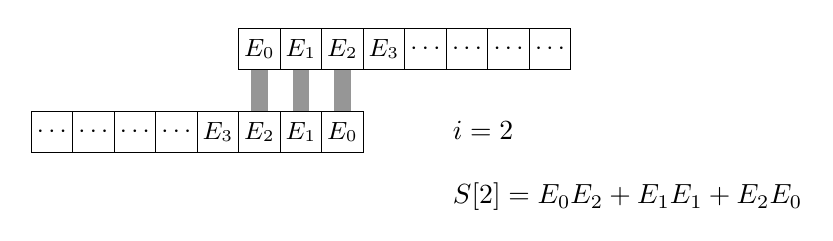
\begin{tikzpicture}[x=0.75pt,y=0.75pt,yscale=-1,xscale=1]
%uncomment if require: \path (0,300); %set diagram left start at 0, and has height of 300

%Shape: Grid [id:dp8843699222147772] 
\draw  [draw opacity=0] (245.47,42) -- (405.47,42) -- (405.47,62) -- (245.47,62) -- cycle ; \draw   (265.47,42) -- (265.47,62)(285.47,42) -- (285.47,62)(305.47,42) -- (305.47,62)(325.47,42) -- (325.47,62)(345.47,42) -- (345.47,62)(365.47,42) -- (365.47,62)(385.47,42) -- (385.47,62) ; \draw    ; \draw   (245.47,42) -- (405.47,42) -- (405.47,62) -- (245.47,62) -- cycle ;
%Shape: Grid [id:dp9924539760633466] 
\draw  [draw opacity=0] (145.47,82) -- (305.47,82) -- (305.47,102) -- (145.47,102) -- cycle ; \draw   (165.47,82) -- (165.47,102)(185.47,82) -- (185.47,102)(205.47,82) -- (205.47,102)(225.47,82) -- (225.47,102)(245.47,82) -- (245.47,102)(265.47,82) -- (265.47,102)(285.47,82) -- (285.47,102) ; \draw    ; \draw   (145.47,82) -- (305.47,82) -- (305.47,102) -- (145.47,102) -- cycle ;
%Straight Lines [id:da33977565845845015] 
\draw [color={rgb, 255:red, 0; green, 0; blue, 0 }  ,draw opacity=0.41 ][line width=6]    (275.47,62) -- (275.47,82) ;
%Straight Lines [id:da5671435028521743] 
\draw [color={rgb, 255:red, 0; green, 0; blue, 0 }  ,draw opacity=0.41 ][line width=6]    (255.47,62) -- (255.47,82) ;
%Straight Lines [id:da7827681813709473] 
\draw [color={rgb, 255:red, 0; green, 0; blue, 0 }  ,draw opacity=0.41 ][line width=6]    (295.47,82) -- (295.47,62) ;

% Text Node
\draw (347.47,85.4) node [anchor=north west][inner sep=0.75pt]    {$i=2$};
% Text Node
\draw (255.47,52) node  [font=\small]  {$E_{0}$};
% Text Node
% Text Node
\draw (295.47,92) node  [font=\small]  {$E_{0}$};
% Text Node
\draw (275.47,52) node  [font=\small]  {$E_{1}$};
% Text Node
\draw (295.47,52) node  [font=\small]  {$E_{2}$};
% Text Node
\draw (275.47,92) node  [font=\small]  {$E_{1}$};
% Text Node
\draw (255.47,92) node  [font=\small]  {$E_{2}$};
% Text Node
\draw (235.47,92) node  [font=\small]  {$E_{3}$};
% Text Node
\draw (315.47,52) node  [font=\small]  {$E_{3}$};
% Text Node
\draw (347.47,115.4) node [anchor=north west][inner sep=0.75pt]    {$S[ 2] =E_{0} E_{2} +E_{1} E_{1} +E_{2} E_{0}$};
% Text Node
\draw (335.47,52) node  [font=\small]  {$\cdots $};
% Text Node
\draw (355.47,52) node  [font=\small]  {$\cdots $};
% Text Node
\draw (375.47,52) node  [font=\small]  {$\cdots $};
% Text Node
\draw (395.47,52) node  [font=\small]  {$\cdots $};
% Text Node
\draw (215.47,92) node  [font=\small]  {$\cdots $};
% Text Node
\draw (195.47,92) node  [font=\small]  {$\cdots $};
% Text Node
\draw (175.47,92) node  [font=\small]  {$\cdots $};
% Text Node
\draw (155.47,92) node  [font=\small]  {$\cdots $};


\end{tikzpicture}

\end{center}

The resultant array $S$ is such that $S[i]\neq 0$ if and only if $i$ is a possible sum.

Return all indices $i$ such that $S[i]\neq 0$.
    
\end{solution}
\end{document}